% Figure 4: Dual-CNI resilience design (two nodes shown)
% Same drawing as in ppt/project2/slides.tex. Compile: pdflatex fig4_cni_architecture.tex
\documentclass[border=4pt]{standalone}
\usepackage{amssymb}
\usepackage{tikz}
\usetikzlibrary{arrows.meta, positioning, fit, backgrounds, calc}
\renewcommand{\familydefault}{\sfdefault}
\tikzset{
  box/.style={draw, rounded corners, align=center, font=\scriptsize,
    minimum width=2.4cm, minimum height=0.6cm},
  arr/.style={-{Stealth[length=1.6mm]}, thick},
  biarr/.style={{Stealth[length=1.6mm]}-{Stealth[length=1.6mm]}, thick},
}
\begin{document}
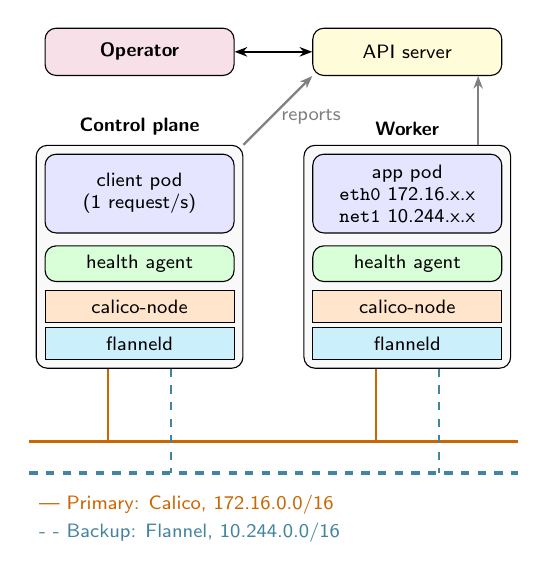
\begin{tikzpicture}[font=\scriptsize]
  \node[box, fill=purple!12] (op) at (0,3.2) {\textbf{Operator}};
  \node[box, fill=yellow!15] (api) at (3.4,3.2) {API server};
  \draw[biarr] (op) -- (api);
  \node[box, fill=blue!10, minimum height=1.0cm] (p1) at (0,1.4) {client pod\\(1 request/s)};
  \node[box, fill=blue!10, minimum height=1.0cm] (p2) at (3.4,1.4) {app pod\\\texttt{eth0} 172.16.x.x\\\texttt{net1} 10.244.x.x};
  \foreach \i/\name in {1/Control plane, 2/Worker} {
    \node[box, fill=green!15, below=0.15cm of p\i, minimum height=0.45cm] (ag\i) {health agent};
    \node[box, fill=orange!20, below=0.1cm of ag\i, minimum height=0.4cm, rounded corners=0pt] (c\i) {calico-node};
    \node[box, fill=cyan!20, below=0.05cm of c\i, minimum height=0.4cm, rounded corners=0pt] (f\i) {flanneld};
    \begin{scope}[on background layer]
      \node[draw, rounded corners, fill=gray!5, fit=(p\i)(f\i), inner sep=3pt,
        label={[font=\scriptsize\bfseries]north:\name}] (n\i) {};
    \end{scope}
  }
  \draw[arr, gray] (n1.north east) -- node[right, pos=0.4]{reports} (api.south west);
  \draw[arr, gray] ([xshift=9mm]n2.north) -- ([xshift=9mm]api.south);
  \draw[very thick, orange!80!black] (-1.4,-1.75) -- (4.8,-1.75);
  \draw[very thick, cyan!60!black, dashed] (-1.4,-2.15) -- (4.8,-2.15);
  \foreach \n in {n1,n2} {
    \draw[orange!80!black, thick] ([xshift=-4mm]\n.south) -- ([xshift=-4mm]\n.south |- 0,-1.75);
    \draw[cyan!60!black, thick, dashed] ([xshift=4mm]\n.south) -- ([xshift=4mm]\n.south |- 0,-2.15);
  }
  \node[anchor=west, orange!80!black] at (-1.4,-2.55) {--- Primary: Calico, 172.16.0.0/16};
  \node[anchor=west, cyan!60!black] at (-1.4,-2.9) {- - Backup: Flannel, 10.244.0.0/16};
\end{tikzpicture}
\end{document}
